\problemname{Wordfeud}
Wordfeud is a Scrabble-like game where you place letter tiles on a grid board to form words. Words can be placed either from left to right or from top to bottom. Each letter gives a certain score. Additionally, there are a number of special squares on the board, which can be of four types:

\begin{itemize}
	\item \texttt{DL} (double letter): the letter score for a tile on this square is doubled
	\item \texttt{TL} (triple letter): the letter score for a tile on this square is tripled
	\item \texttt{DW} (double word): the score for the entire word is doubled if the square is covered
	\item \texttt{TW} (triple word): the score for the entire word is tripled if the square is covered
\end{itemize}

When computing the score for a word, you start by summing the letter scores, with any multiplication applied to each letter. Once the sum is computed, it is multiplied by any word multipliers. Note that if the word covers multiple \texttt{DW} or \texttt{TW} squares, the score can be multiplied several times.

In this problem, we consider an empty $10$x$10$ board where the rows and columns are numbered according to the figure. Write a program that, given the placement of special squares on the board and the word you intend to place, computes the highest score you can get if you may place the word wherever you want (but entirely within the board).

\begin{figure}[!h]
	\centering
	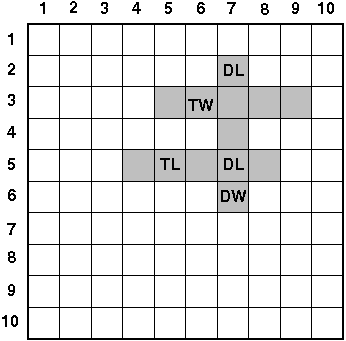
\includegraphics[width=0.35\textwidth]{wordfeud}
	\caption{The board in the example with the special squares marked. The shaded areas show three examples of placement of the ``word'' $56141$. The vertical placement gives $2\cdot(2\cdot5+6+1+2\cdot4+1)=52$ points, the horizontal one on row $3$ gives $51$ points, and the horizontal one on row $5$ gives $33$ points.}
\end{figure}

\section*{Input}
The first line contains $N$ ($1\leq N \leq 10$), the number of special squares.

The following $N$ lines each describe a special square. Each square consists of two numbers, the row and
column of the special square (both in the range $1$ to $10$), and the type of the special square (\texttt{DL}, \texttt{TL}, \texttt{DW}, or \texttt{TW}).

Finally follows one last line, containing the word to be placed. For simplicity, each letter has already been replaced with its point value, a digit between $0$ and $8$. The word can have up to $7$ letters.

\section*{Output}
Output an integer: the maximum score possible for the given word.

\section*{Scoring}
Your solution will be tested on a set of test groups.
To earn points for a group, you must pass all test cases in that group.

\noindent
\begin{tabular}{| l | l | p{12cm} |}
  \hline
  \textbf{Group} & \textbf{Points} & \textbf{Constraints} \\ \hline
  $1$    & $50$          & \texttt{DW} and \texttt{TL} do not appear in the input.  \\ \hline
  $2$    & $50$          & No additional constraints.  \\ \hline
\end{tabular}
